\documentclass{beamer}
\mode<presentation>

\setbeamertemplate{navigation symbols}{}
\setbeamertemplate{theorems}[numbered]
\setbeamertemplate{items}[default]
\setbeamercovered{dynamic}
\setlength{\unitlength}{1cm}
\setbeamertemplate{footline}[frame number]

\usepackage{setspace}
\usepackage{amsmath,amssymb}
\usepackage{amsthm}
\usepackage{pgf,pgfarrows}
\usepackage[utf8]{inputenc}
% \usepackage[polish]{babel}
\usepackage{polski}
\usepackage{graphics}
\usepackage{tikz}
\usepackage[ruled]{algorithm}
\usepackage{algpseudocode}
\usepackage{scalefnt}
\usepackage{array}
\usepackage{colortbl}
\usepackage{float}
\usepackage{wrapfig}

\usetikzlibrary{arrows,automata,snakes}
\usetheme{Frankfurt}
\usecolortheme{seahorse} %crane
\useinnertheme{circles}


\newtheorem*{lemat}{Lemat}
\newtheorem{twierdzenie}{Twierdzenie}
\newcommand{\myitem}{\item[$\vartriangleright$]}
\newcommand{\nota}[1]{{\color{gray} \emph{#1}}}
\newcommand{\HarmonicN}[1]{H_{#1}}
\newcommand{\BALL}[2]{\mathbf{B}(#1,#2)}
\newcommand{\DISC}[2]{\mathbf{D}(#1,#2)}
\newcommand{\SPHERE}[2]{\mathbf{S}(#1,#2)}
\newcommand{\BigO}[1]{\mathcal{O}\left(#1\right)}
\newcommand{\BigTh}[1]{\Theta\left(#1\right)}
\newcommand{\slfrac}[2]{\left.#1\middle/#2\right.}
\newcommand{\PR}[1]{\mathrm{Pr}\left[#1\right]}
\newcommand{\E}[1]{\mathbb{E}\left[#1\right]}
\newcommand{\var}[1]{\mathbb{V}\mathrm{ar}\left[#1\right]}
\newcolumntype{C}{>{\centering\arraybackslash}p{0.5cm}}
\newcolumntype{Y}{>{\columncolor{blue!5}}C}

%\pgfpagesuselayout{4 on 1 with notes}[a4paper,border shrink=3mm]


\title{Bot do komputerowej gry wyścigowej}

\author{
	\textbf{Kamil Matejuk}
	\newline \newline
	Praca napisana pod kierunkiem \newline \textbf{dra Marcina Michalskiego}
}

\date{Styczeń 2022, Wrocław}


\begin{document}

\begin{frame}[plain]{}
	\titlepage
\end{frame}


\section{Wprowadzenie}
\begin{frame}{Cel i zakres pracy}

	\begin{itemize}
		\myitem Stworzenie gry wyścigowej 3D
		\myitem Stworzenie bota do gry
		\myitem Dokładniejsze poznanie silnika Unity, C\# oraz teorii Reinforcement Learning
	\end{itemize}

\end{frame}

\begin{frame}{Wybór środowiska}

	\begin{itemize}
		\myitem Darmowy silnik do tworzenia gier 3D
		\myitem Wsparcie dla wielu platform (PC, mobile, VR, etc)
		\myitem Jedno z najpopularnijszych rozwiązań na rynku (poza Unreal\textregistered)
		\myitem Niższa bariera wejścia niż Unreal\textregistered
	\end{itemize}

	\vspace{2cm}
	{\hspace*{5cm}
\includegraphics[width=5cm]{figures/Unity_logo.png}}

\end{frame}


\section{Stworzenie gry}
\begin{frame}{Cel gry}

	\begin{itemize}
		\myitem Środowisko testowe dla bota
		\myitem Generator losowych terenów
		\myitem Gra single/multiplayer
	\end{itemize}

	\begin{figure}[!htb]
		\minipage{0.5\textwidth}
			\centering
			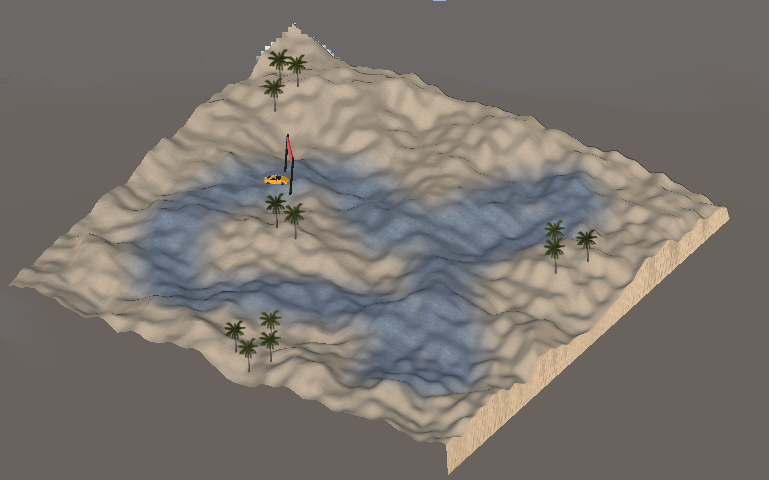
\includegraphics[height=3cm]{figures/terrains_2.png}
		\endminipage\hfill
		\minipage{0.5\textwidth}
			\centering
			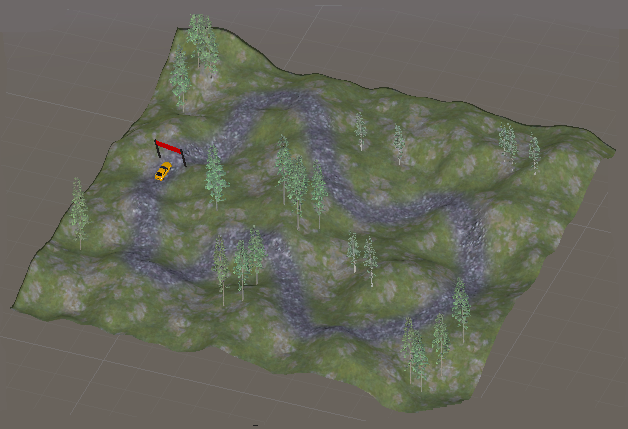
\includegraphics[height=3cm]{figures/terrains_1.png}
		\endminipage
		\end{figure}

\end{frame}

\begin{frame}{Pętla}

	% \begin{itemize}
	% 	\myitem Wybór losowych punktów
	% 	\myitem Posortowanie punktów zgodnie z ruchem wskazówek zegara
	% 	\myitem Wybranie dodatkowych punktów kontrolnych
	% 	\myitem Połączenie punktów z wykorzystaniem krzywej Bezier 3 stopnia
	% \end{itemize}
	
	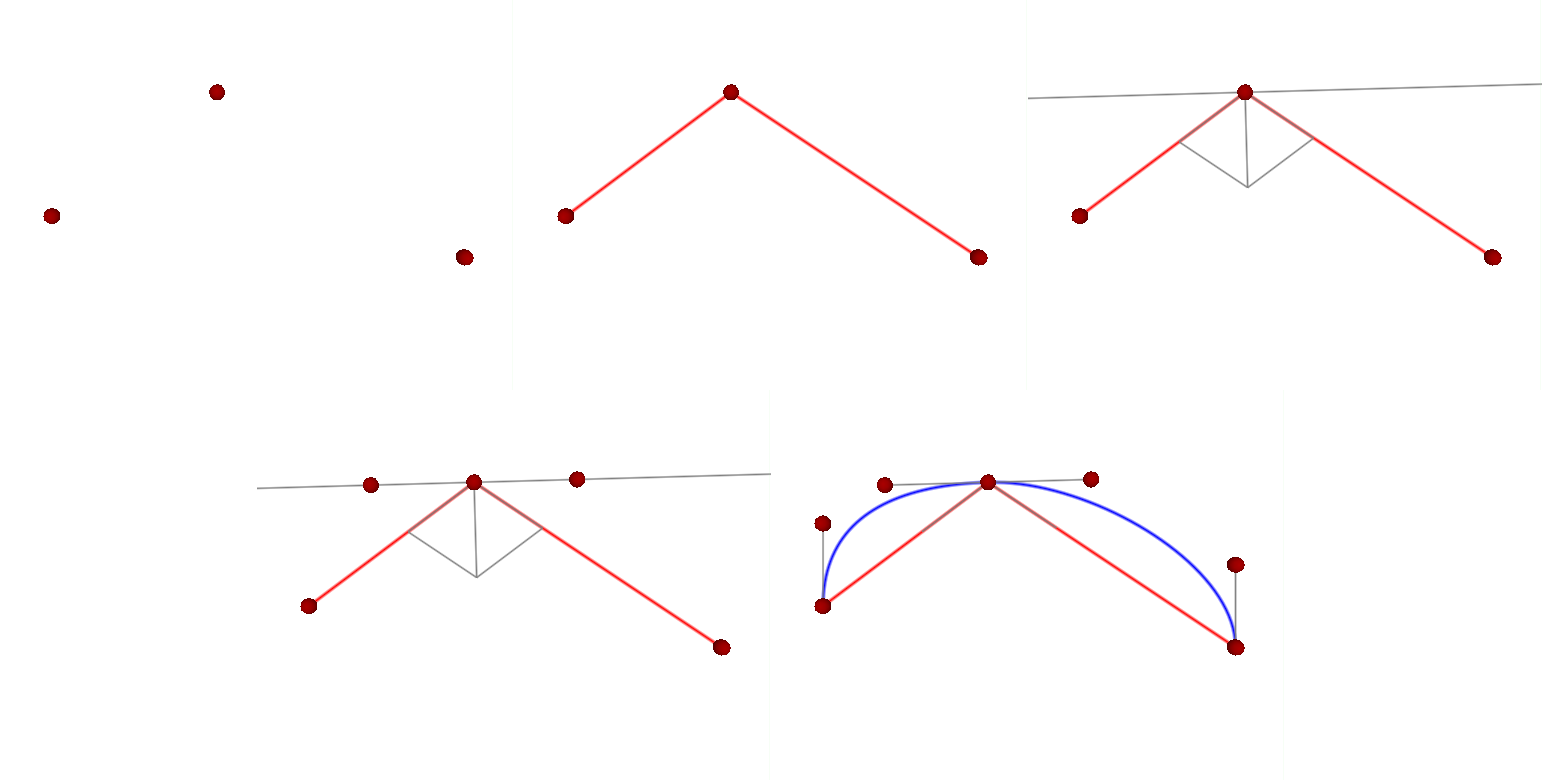
\includegraphics[width=\linewidth]{figures/loop_creation.png}

	% \vspace{2cm}
	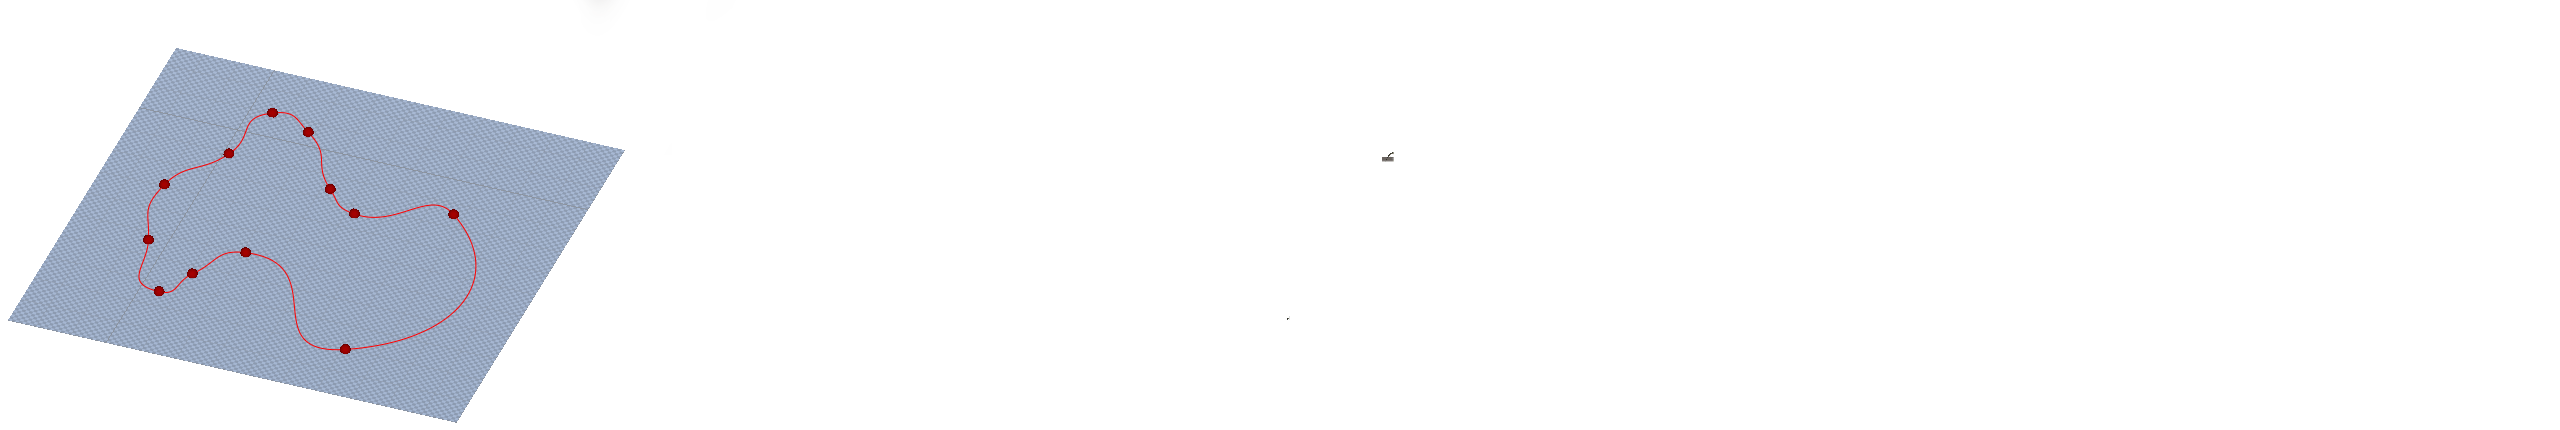
\includegraphics[width=\linewidth]{figures/terrain_creation_1_2.png}

\end{frame}

\begin{frame}{Teren}

	\algrenewcommand\algorithmicrequire{\underline{\textsc{height(x, y)}}}
	\texttt{
	\begin{algorithmic}[1]
		\Require
		\Statex x $\gets$ (x + offset) * scale
		\Statex y $\gets$ (y + offset) * scale
		\Statex r1 $\gets$ detailsMain * Mathf.PerlinNoise(x/2, y/2)
		\Statex r2 $\gets$ detailsMinor * Mathf.PerlinNoise(x, z)
		\Statex r3 $\gets$ detailsTiny * Mathf.PerlinNoise(x*2, z*2)
		\Statex \Return r1 + r2 + r3
	\end{algorithmic}}

	\vspace{1cm}
	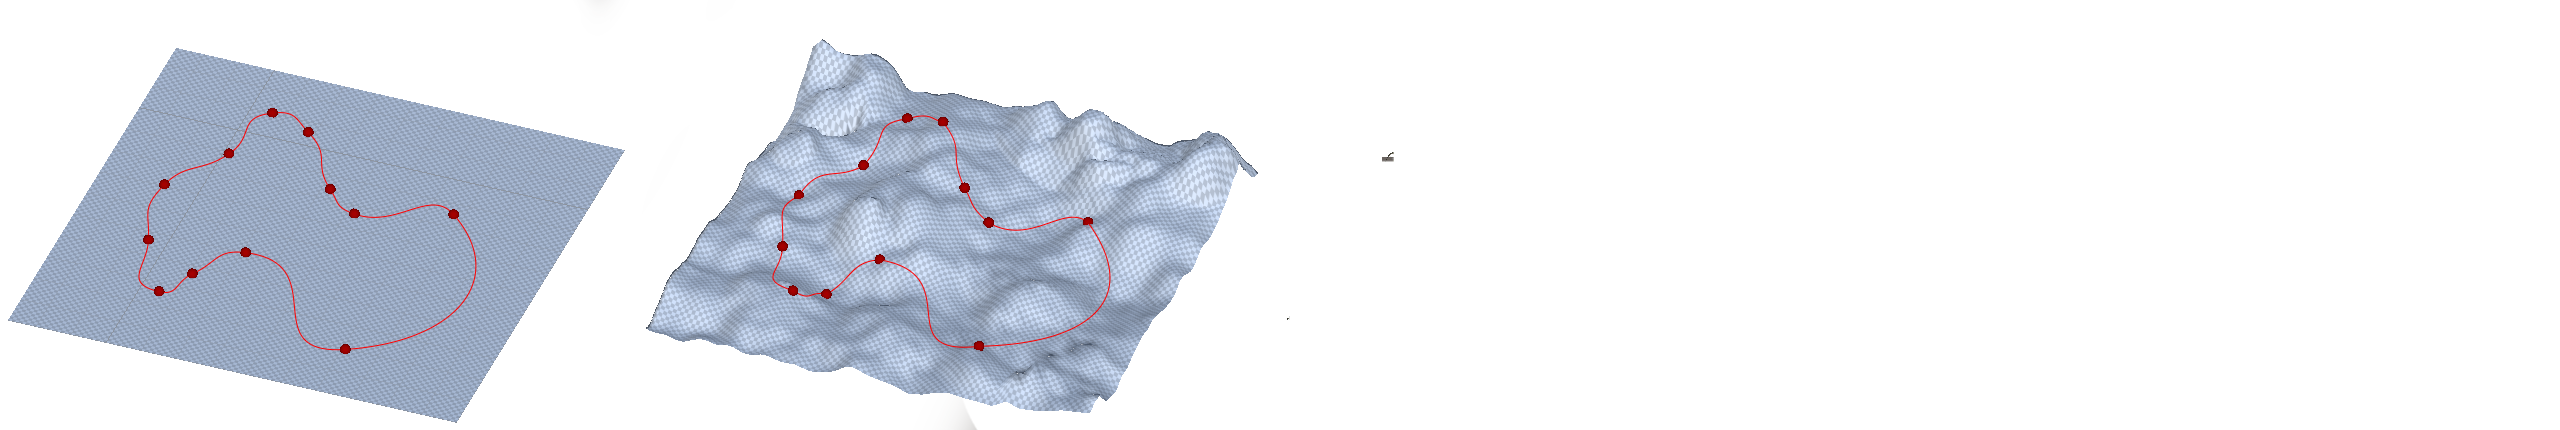
\includegraphics[width=\linewidth]{figures/terrain_creation_2_2.png}

\end{frame}

\begin{frame}[fragile]{Tekstury}

	\begin{columns}
		\begin{column}{.6\hsize}
			\algrenewcommand\algorithmicrequire{\underline{\textsc{}}}
			\texttt{
			\begin{algorithmic}[1]
				\Require
				\Statex texture (
					\Statex \hskip2em float height,
					\Statex \hskip2em Vector3 normal,
					\Statex \hskip2em float steepness,
					\Statex \hskip2em float distanceToRoad
				\Statex ) \{ ... \}
			\end{algorithmic}}
		\end{column}

		\begin{column}{.4\hsize}
			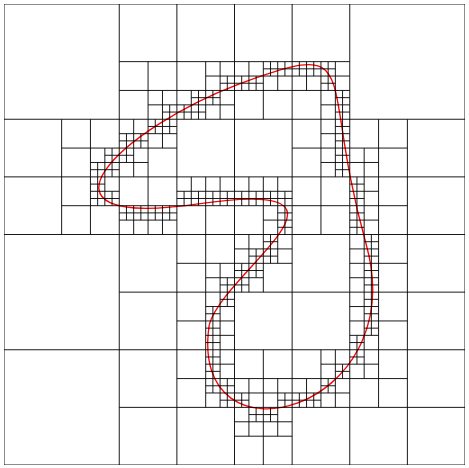
\includegraphics[width=\linewidth]{figures/terrain_subdivision_for_road.png}
		\end{column}
	\end{columns}

	\vspace{1cm}
	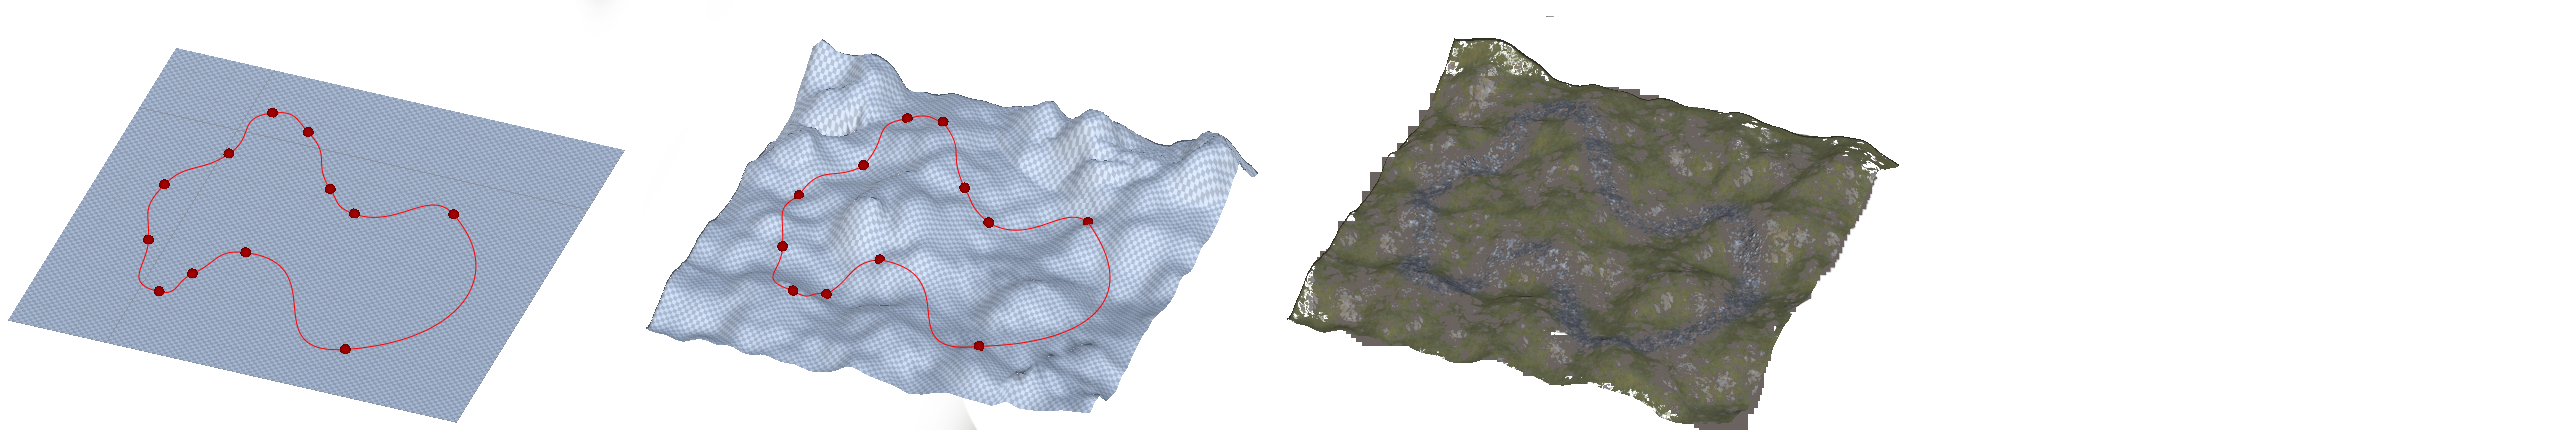
\includegraphics[width=\linewidth]{figures/terrain_creation_3_2.png}

\end{frame}

\begin{frame}{Obiekty}

	\begin{columns}

		\begin{column}{.55\hsize}
			\begin{itemize}
				\myitem Start / Meta
				\myitem Pojazdy
				\myitem Elementy otoczenia
			\end{itemize}
		\end{column}
		
		\begin{column}{.45\hsize}
			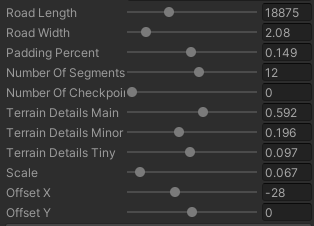
\includegraphics[width=\linewidth]{figures/terrain_gen_params.png}
		\end{column}

	\end{columns}

	\vspace{1.5cm}
	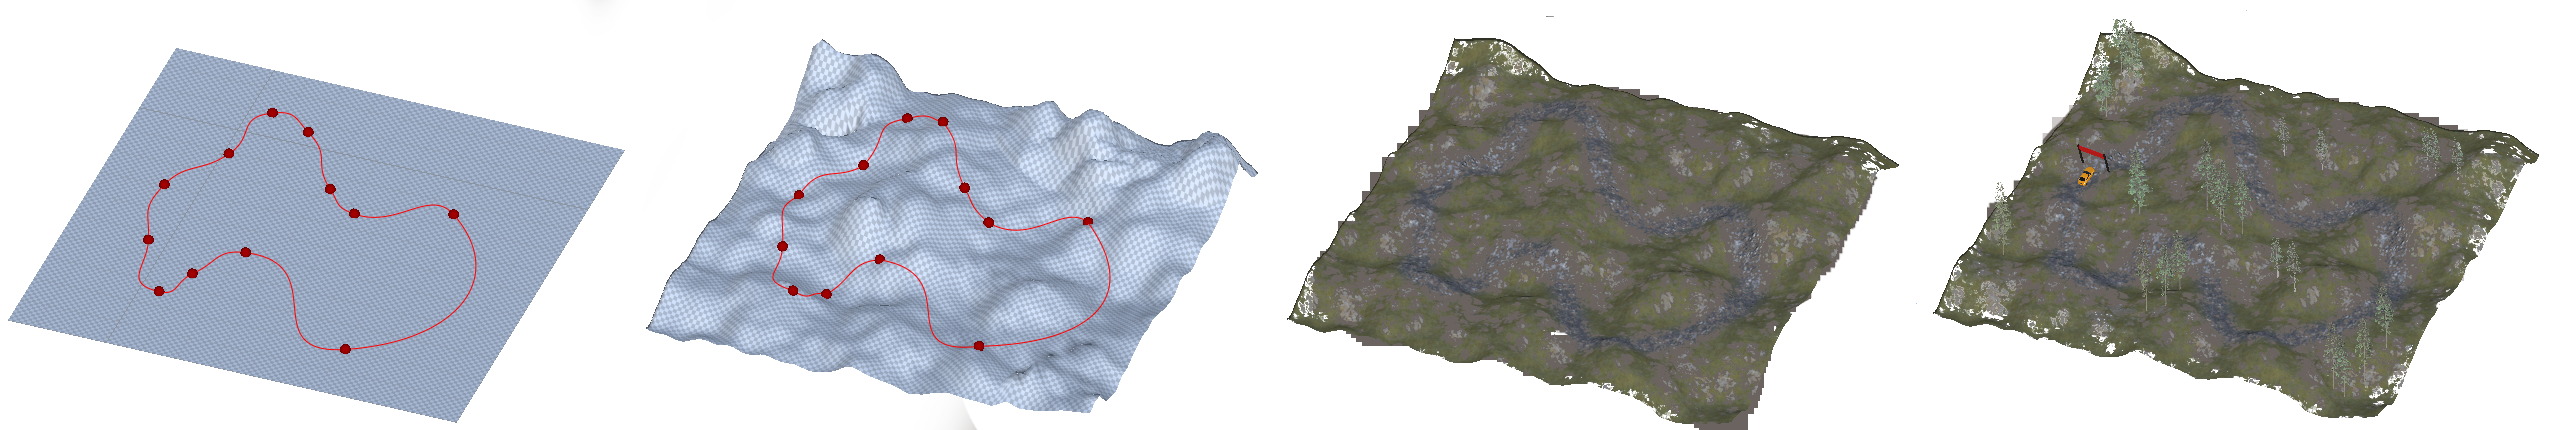
\includegraphics[width=\linewidth]{figures/terrain_creation_4_2.png}

\end{frame}


\section{Stworzenie bota}
\begin{frame}{Reinforcement learning}
	
	\begin{center}
		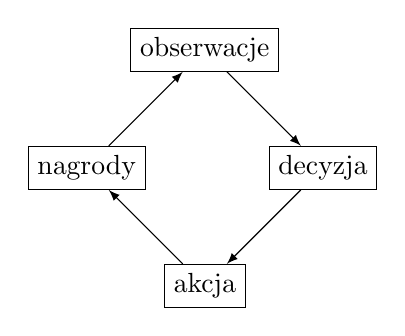
\begin{tikzpicture}
			\node[draw] at (0, 1.5) (1) {obserwacje};
			\node[draw] at (1.5, 0) (2) {decyzja};
			\node[draw] at (0, -1.5) (3) {akcja};
			\node[draw] at (-1.5, 0) (4) {nagrody};
			\draw [->,-latex] (1) to (2);
			\draw [->,-latex] (2) to (3);
			\draw [->,-latex] (3) to (4);
			\draw [->,-latex] (4) to (1);
		\end{tikzpicture}
	\end{center}
	
\end{frame}

% \begin{frame}{Technologie}

	\begin{columns}

		\begin{column}{.4\hsize}
			\textbf{Unity MLAgents}
			\begin{itemize}
				\myitem Tensorflow
				\myitem Tensorboard
			\end{itemize}
		\end{column}
		
		\begin{column}{.6\hsize}
			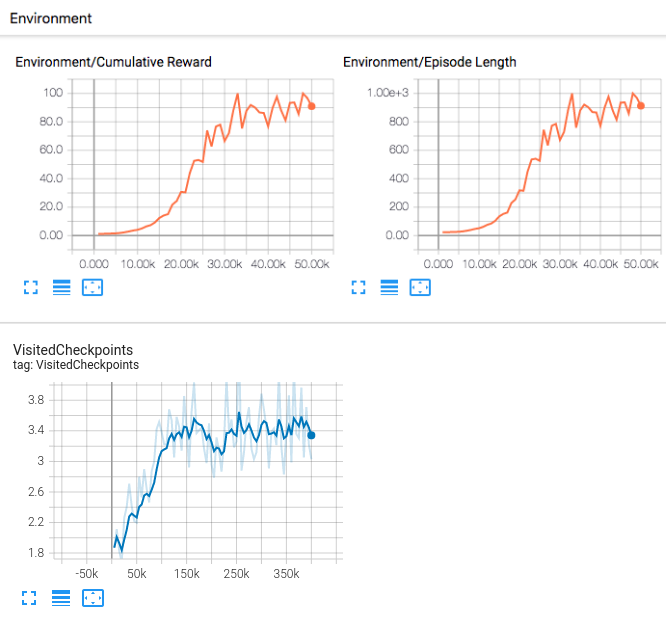
\includegraphics[width=\linewidth]{figures/tensorboard.png}
		\end{column}

	\end{columns}

\end{frame}

\begin{frame}{Podjęcie akcji}
	
	\begin{columns}
		\begin{column}{.8\hsize}
			\textbf{ruch przód/tył oraz skręt kierownicy}
			\begin{itemize}
				\myitem wartości dyskretne $\{-1, 0, 1\}$
				\myitem wartości ciągłe $[-1, 1]$
			\end{itemize}
			
			\vspace{1cm}
			{\hspace*{2cm}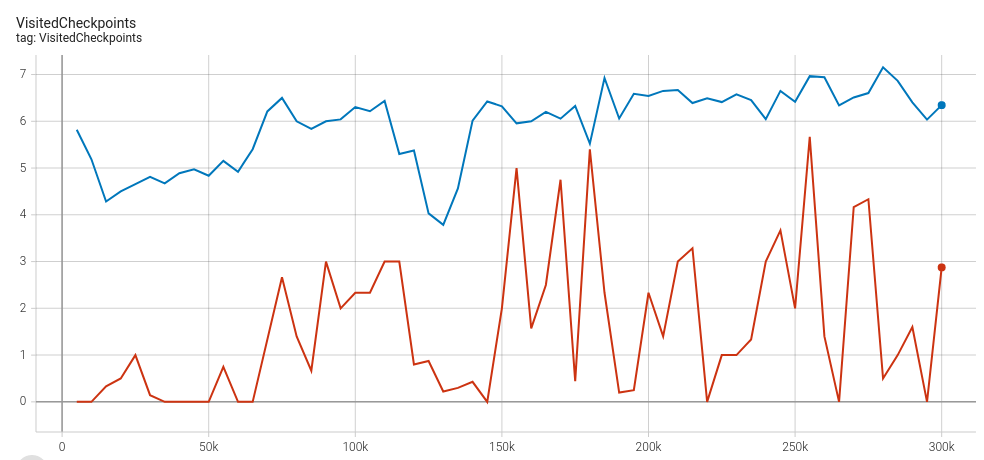
\includegraphics[width=.8\linewidth]{figures/output_values_compare.png}}
		\end{column}

		\begin{column}{.2\hsize}
			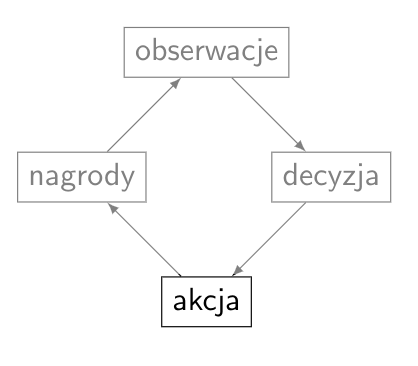
\includegraphics[width=\linewidth]{figures/learning_loop_3.png}
			\vspace{5cm}
		\end{column}
	\end{columns}
	
\end{frame}

\begin{frame}{Ocena akcji}

	\begin{columns}
		\begin{column}{.65\hsize}
			\textbf{Po każdej akcji:}
			\begin{itemize}
				\myitem (0.3 - distanceToRoadCenter) * 0.01
				\myitem (distanceTraveledInFrame - 0.1) * 0.1
				\myitem (0.07 - abs(angleToTangent)) * 0.1
			\end{itemize}
			\vspace{5cm}
		\end{column}
		
		\begin{column}{.5\hsize}
			{\hspace*{.6\linewidth}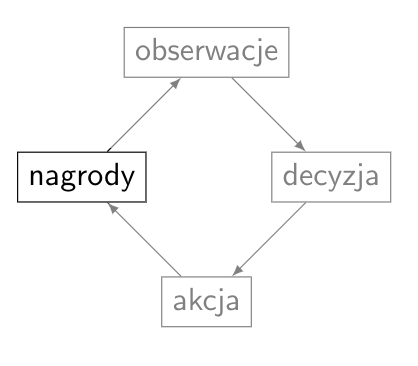
\includegraphics[width=.4\linewidth]{figures/learning_loop_4.png}}
			\vspace{7cm}
			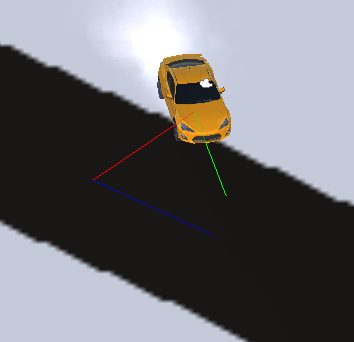
\includegraphics[width=\linewidth]{figures/rewards.png}
		\end{column}
	\end{columns}
	
\end{frame}

\begin{frame}{Ocena akcji}
	
	\begin{columns}
		\begin{column}{.5\hsize}
			\textbf{Przy kolizji:}
			\begin{itemize}
				\myitem z kolejnym checkpointem $+1$
				\myitem z innym checkpointem $-0.1$
				\myitem z krawędzią pola $-0.1$
			\end{itemize}
			\vspace{1cm}
			\textbf{Zakończenie epizodu po kolizji z krawędzą terenu/drogi}
			\vspace{3cm}
		\end{column}
		
		\begin{column}{.5\hsize}
			{\hspace*{.6\linewidth}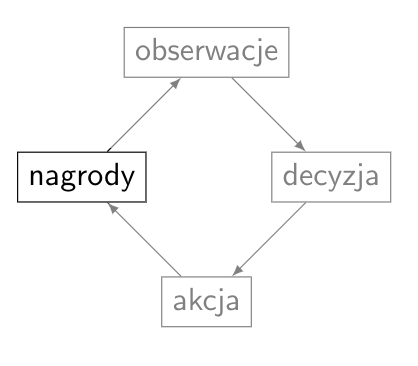
\includegraphics[width=.4\linewidth]{figures/learning_loop_4.png}}
			\vspace{7cm}
			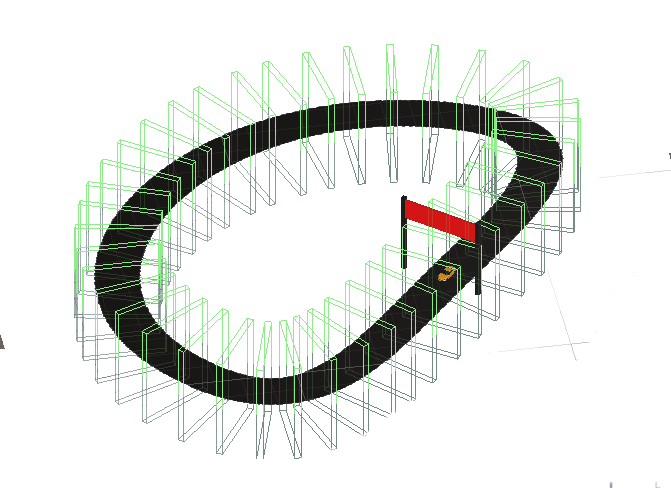
\includegraphics[width=\linewidth]{figures/checkpoints.png}
		\end{column}
	\end{columns}
	
\end{frame}

\begin{frame}{Wybór obserwacji}
	
	\begin{columns}
		\begin{column}{.8\hsize}
			\textbf{Obserwacje:}
			\begin{itemize}
				\myitem dane pobrane bezpośrednio z równania trasy
				\myitem kolory na około pojazdu
				\myitem widok z kamery (perspektywa pierwszosobowa)
				\myitem widok z kamery (perspektywa lotu ptaka)
			\end{itemize}
			\vspace{1cm}
		\end{column}
		
		\begin{column}{.2\hsize}
			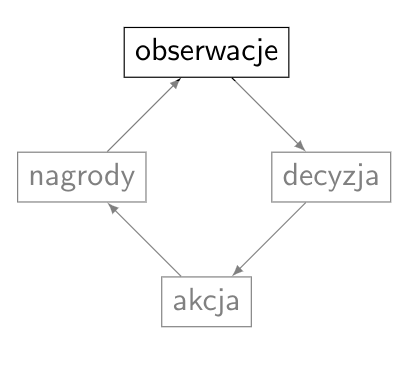
\includegraphics[width=\linewidth]{figures/learning_loop_1.png}
			\vspace{2cm}
		\end{column}
	\end{columns}

	\begin{columns}
		\begin{column}{.3\hsize}
			\centering
			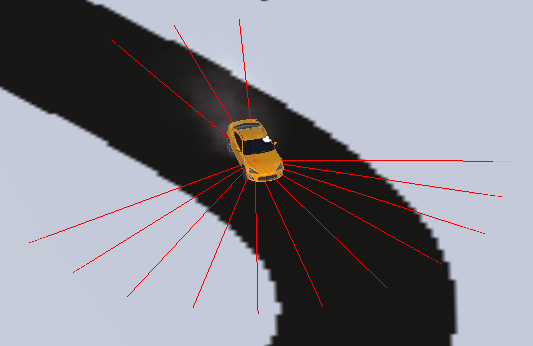
\includegraphics[width=\linewidth]{figures/observations_1.png}
			(1, 14)
		\end{column}
		\begin{column}{.3\hsize}
			\centering
			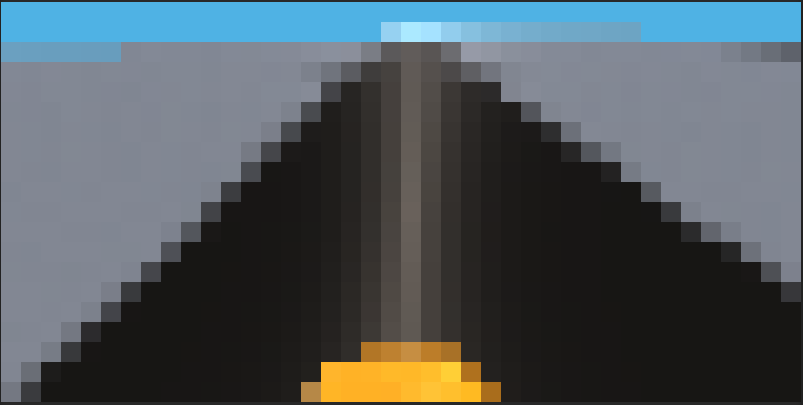
\includegraphics[width=\linewidth]{figures/observations_2.png}
			(40, 20)
		\end{column}
		\begin{column}{.3\hsize}
			\centering
			
\includegraphics[width=\linewidth]{figures/observations_3.png}
			(30, 20)
		\end{column}
	\end{columns}
	
\end{frame}

\begin{frame}{Wyniki}
	
	\begin{columns}
		\begin{column}{.5\hsize}
			\textbf{Porównanie treningu }
			\begin{itemize}
				\myitem niebieski - widok z kamery z lotu ptaka
				\myitem czerwony - dane trasy
			\end{itemize}
			\vspace{1cm}
		\end{column}

		\begin{column}{.5\hsize}
			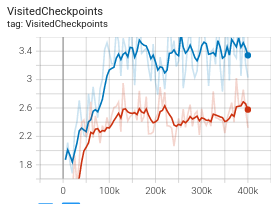
\includegraphics[width=\linewidth]{figures/compare_res_1_checkpoints.png}
		\end{column}
	\end{columns}

	\begin{columns}
		\begin{column}{.5\hsize}
			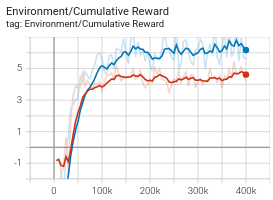
\includegraphics[width=\linewidth]{figures/compare_res_1_rewards.png}
		\end{column}
		\begin{column}{.5\hsize}
			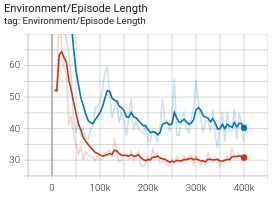
\includegraphics[width=\linewidth]{figures/compare_res_1_length.png}
		\end{column}
	\end{columns}
	
\end{frame}

\begin{frame}{Dobranie hiperparametrów}

	% \begin{columns}
	% 	\begin{column}{.25\hsize}
	% 		\begin{itemize}
	% 			\myitem batch size
	% 			\myitem buffer size
	% 		\end{itemize}
	% 	\end{column}

	% 	\begin{column}{.3\hsize}
	% 		\begin{itemize}
	% 			\myitem learning rate
	% 			\myitem num epoch
	% 		\end{itemize}
	% 	\end{column}
		
	% 	\begin{column}{.25\hsize}
	% 		\begin{itemize}
	% 			\myitem beta
	% 			\myitem epsilon
	% 		\end{itemize}
	% 	\end{column}
		
	% 	\begin{column}{.25\hsize}
	% 		\begin{itemize}
	% 			\myitem lambd
	% 			\myitem gamma
	% 		\end{itemize}
	% 	\end{column}
	% \end{columns}

	\begin{columns}
		\begin{column}{\hsize}
			% \hspace*{3.9cm}
			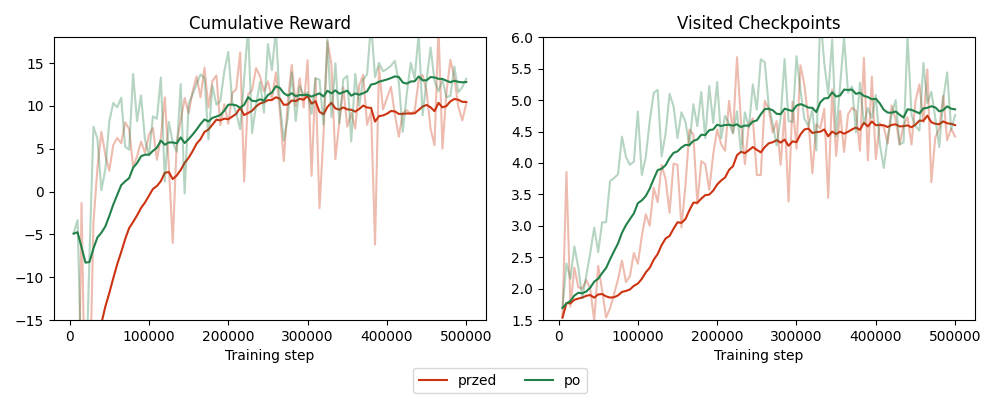
\includegraphics[width=\linewidth]{figures/hyperparameters_tuning_results.png}
		\end{column}
	\end{columns}

	\begin{table}[H]
		\centering
		\resizebox{\textwidth}{!}{%
		\begin{tabular}{|c|c|c|c|c|c|c|}
			\hline
			& \multicolumn{3}{c|}{Funkcja nagrody} & \multicolumn{3}{c|}{Postęp trasy}\\
			& przed & po & zmiana & przed & po & zmiana \\
			\hline
			\hline
			średnia z wszystkich iteracji       &  7.38 &  9.79 & +32.5\% & 3.91 & 4.49 & +14.8\% \\
			średnia z najlepszych 99\% iteracji &  7.81 & 10.15 & +29.9\% & 3.93 & 4.52 & +15.0\% \\
			średnia z najlepszych 90\% iteracji &  9.63 & 11.49 & +19.3\% & 4.15 & 4.73 & +13.9\% \\
			średnia z najlepszych 50\% iteracji & 12.38 & 13.99 & +13.0\% & 4.75 & 5.13 &  +8.0\% \\
			maksimum                            & 19.04 & 19.64 &  +3.1\% & 6.18 & 6.35 &  +2.7\% \\
			\hline
		\end{tabular}
	}
	\end{table}

\end{frame}


\section{Podsumowanie}
\begin{frame}{Trening}

	\begin{columns}
		\begin{column}{.7\hsize}

			\begin{table}[H]
				\centering
				\resizebox{\textwidth}{!}{%
				\begin{tabular}{|c|c|c|c|c|c|c|}
					\hline
					& \multicolumn{6}{c|}{Wynik bota po N-tym etapie treningu}\\
					Numer toru & po 1 etapie & po 2 etapie & po 3 etapie & po 4 etapie & po 5 etapie & po 6 etapie \\
					\hline
					\hline
					1 & 100\% & 100\% & 100\% & 100\% & 100\% & 100\% \\
					2 & 0\% & 33\% & 0\% & 33\% & 33\% & 100\% \\
					3 & 100\% & 100\% & 33\% & 100\% & 33\% & 100\% \\
					4 & 100\% & 100\% & 0\% & 100\% & 33\% & 100\% \\
					5 & 0\% & 33\% & 100\% & 100\% & 33\% & 100\% \\
					6 & 0\% & 0\% & 0\% & 33\% & 33\% & 66\% \\
					7 & 0\% & 0\% & 0\% & 0\% & 0\% & 66\% \\
					8 & 33\% & 0\% & 0\% & 0\% & 0\% & 33\% \\
					\hline
				\end{tabular}}
			\end{table}

		\end{column}
		\begin{column}{.4\hsize}
			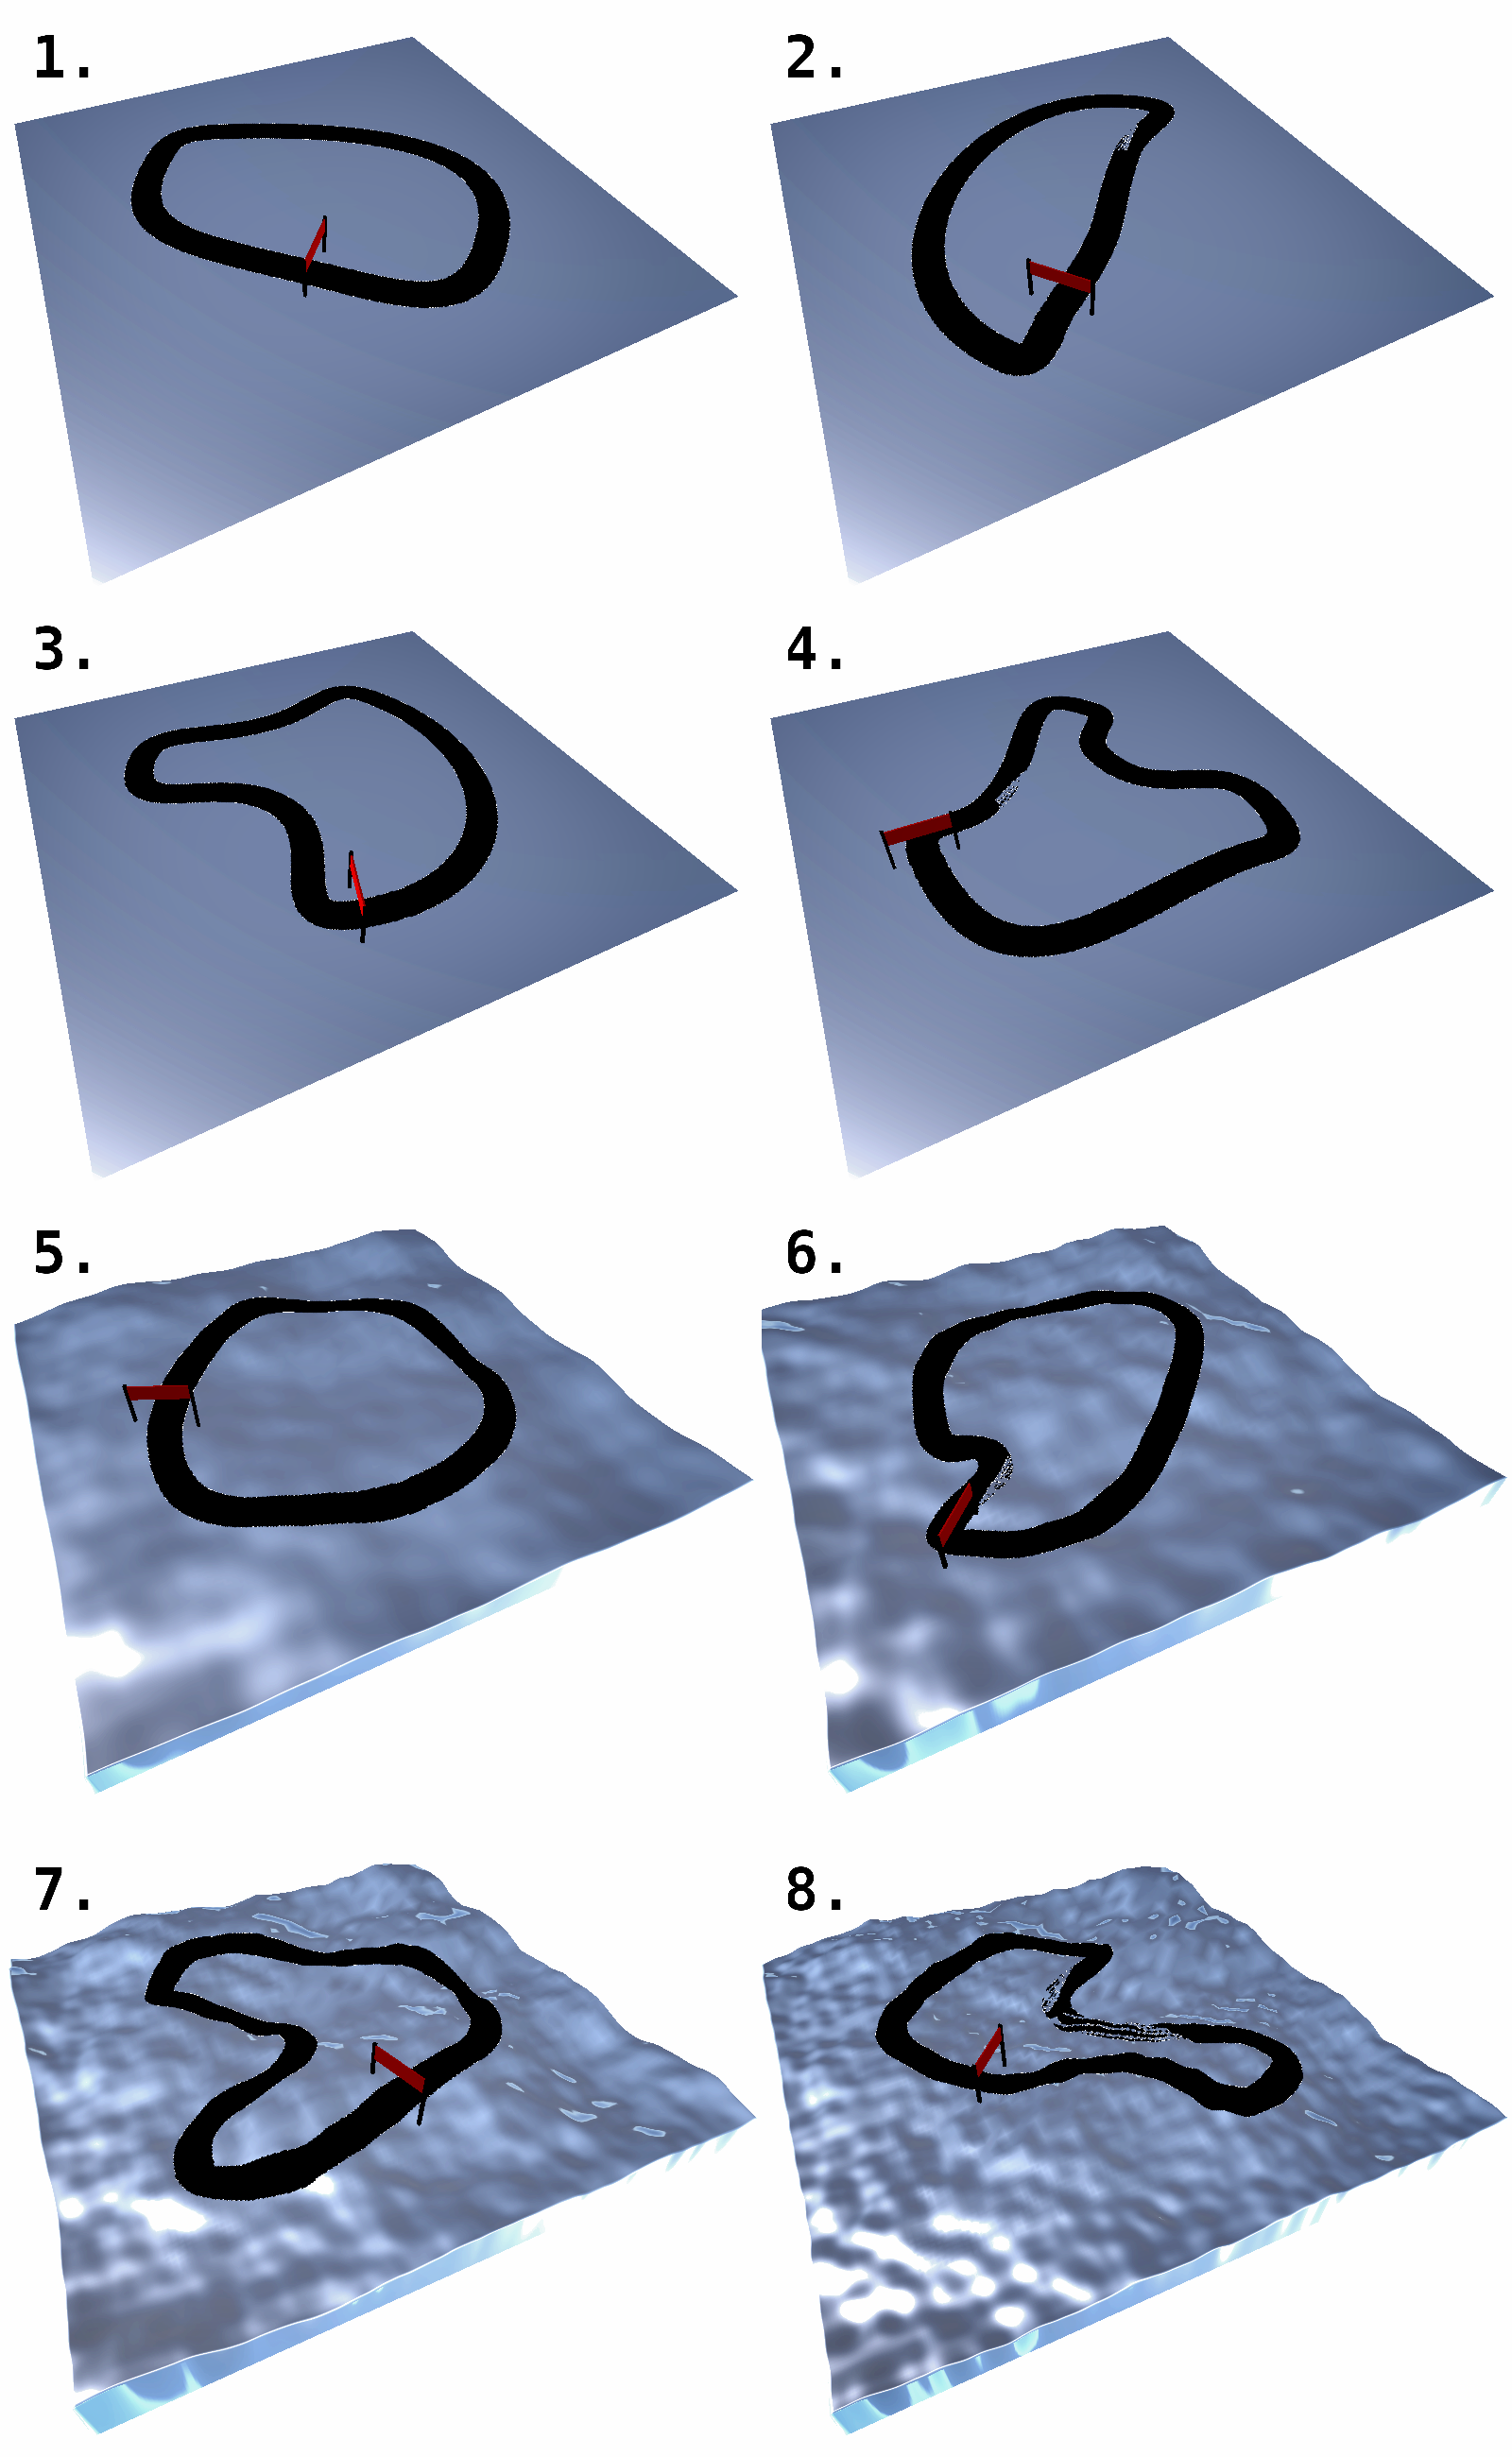
\includegraphics[width=\linewidth]{figures/trening_environs.png}
		\end{column}
	\end{columns}

\end{frame}


\begin{frame}{}
	\begin{center}
		\large{Dziękuję za uwagę.}
	\end{center}
\end{frame}

\end{document} 